\chapter{Appendix}

\section{Age Histogram}
\label{app:age_hist}

Figure~\ref{fig:app_age_hist} shows an age distribution of 522 stars in the
catalog with an existing age value.

\begin{figure}[h!]
    \centering
    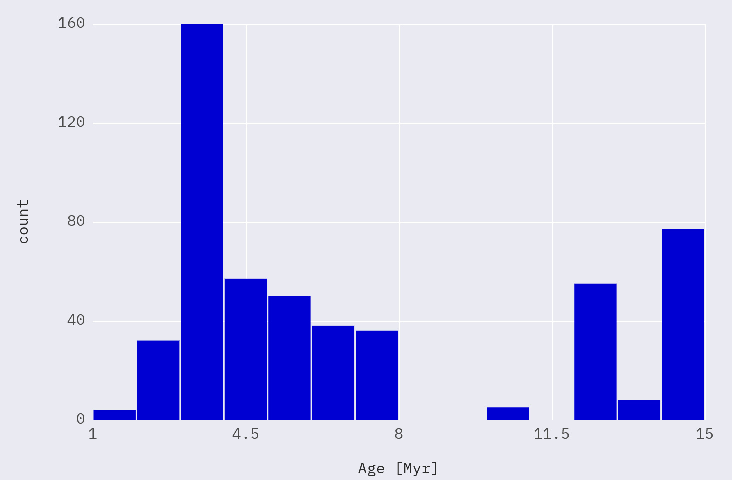
\includegraphics[width=0.6\linewidth]{figures/age_hist.pdf}
    \caption{}
    \label{fig:app_age_hist}
\end{figure}


\section{Velocity Vector Visualizations}
\label{app:vectorplots}

Figure~\ref{fig:app_uvw_vectors} shows the full three-dimensional velocity vectors
$(U, V, W)$ of the subsample of 180 stars for which a radial-velocity measurement is
available, plotted at their respective three-dimensional positions within the
reconstruction volume. Figure~\ref{fig:app_pm_vectors} instead shows the tangential
proper-motion vectors of the full 557-star catalog, projected onto the plane of the sky
as seen from the Sun; since these are angular rather than physical velocities, no
distance information is encoded in this second plot.

\begin{figure}[h!]
    \centering
    \begin{subfigure}[b]{0.9\linewidth}
        \centering
        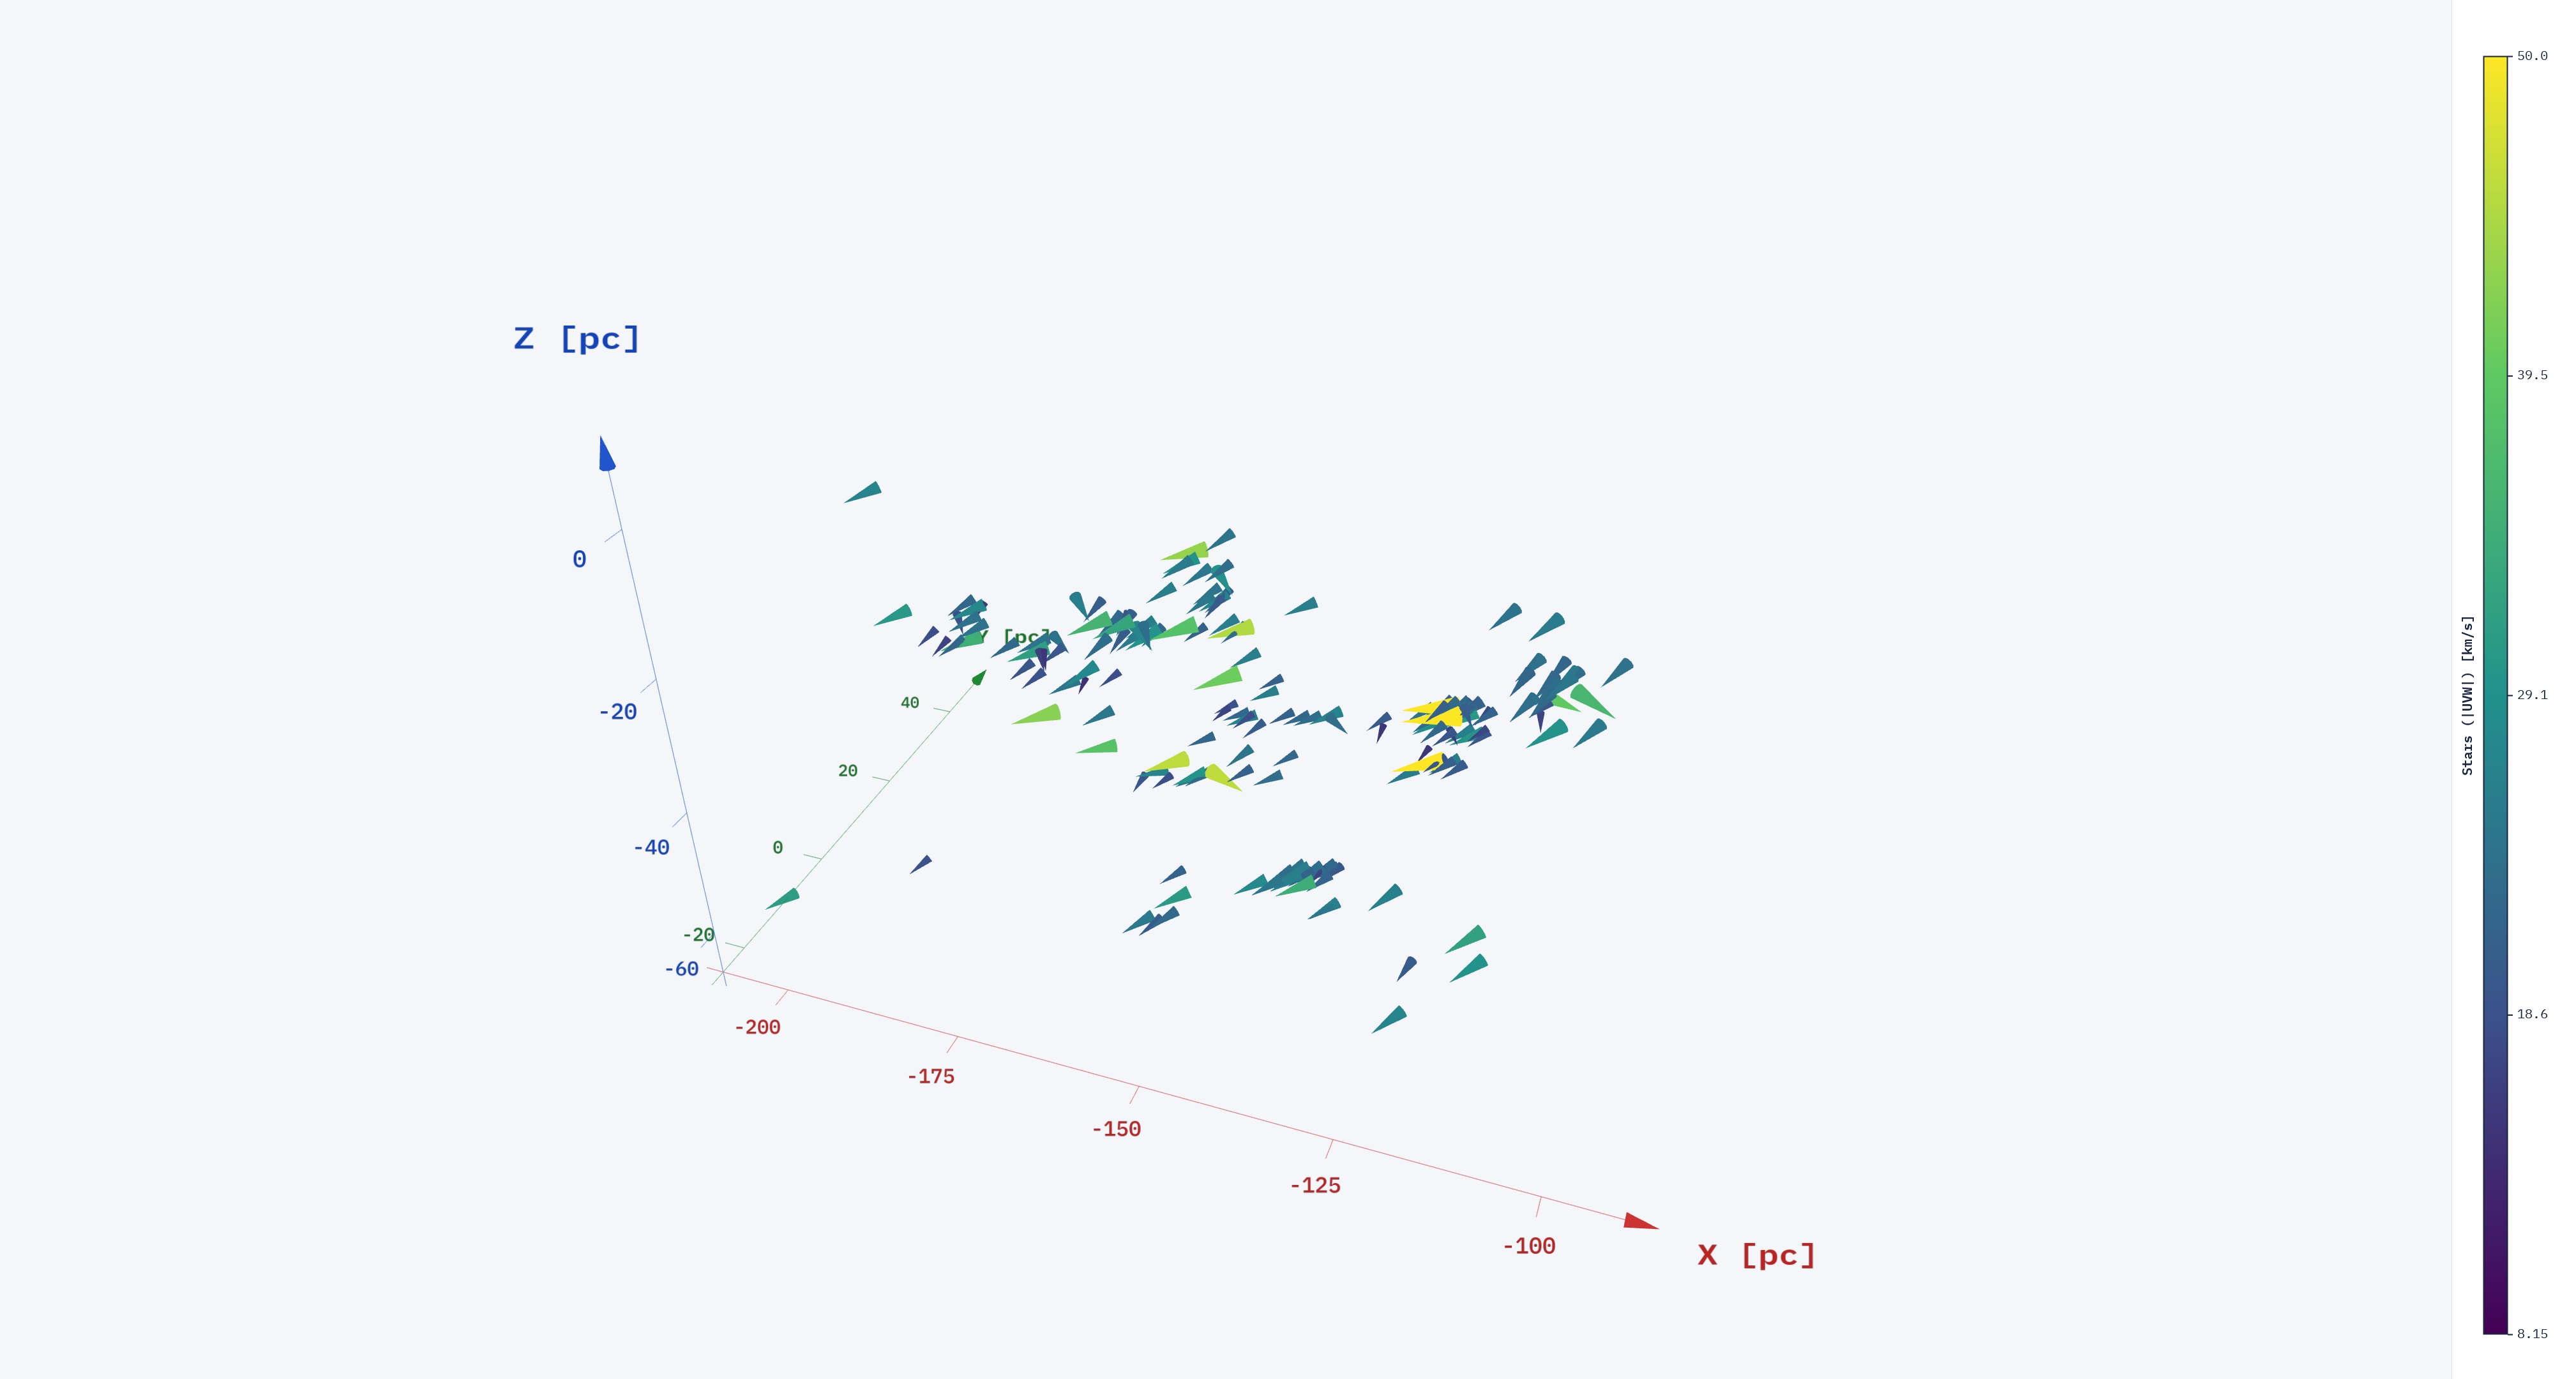
\includegraphics[width=\linewidth]{figures/UVW.png}
        \caption{Full three-dimensional velocity vectors of the radial-velocity
            subsample, shown at their three-dimensional positions.}
        \label{fig:app_uvw_vectors}
    \end{subfigure}
    \vspace{1em}
    \begin{subfigure}[b]{0.9\linewidth}
        \centering
        
\includegraphics[width=\linewidth]{figures/test.png}
        \caption{Proper-motion vectors of the full catalog, projected onto the sky.}
        \label{fig:app_pm_vectors}
    \end{subfigure}
    \caption{Vector-based illustrations of the two velocity data modalities entering the
        reconstruction: full three-dimensional space velocities of the radial-velocity
        subsample (top) versus sky-projected proper motions of the full sample (bottom).}
    \label{fig:app_vectors}
\end{figure}